\subsection{Lessenrooster - FR5}

%Richting Bekijken 
\subsubsection{Richting Bekijken}   
\noindent\begin{table}[H]
            \begin{tabular}{l | p{10cm}}
                \textbf{ID:} & FR5.1 \\ \hline
                \textbf{TITEL:} & Lesrooster van richting bekijken \\ \hline
                \textbf{PRIORITEIT:} &  Hoog \\ \hline
                \textbf{PREREQUISITIES:} & \\ \hline
                \textbf{TOEGANG:} &  Iedereen \\ \hline
                \textbf{BESCHRIJVING:} & Een (niet) ingelogde gebruiker heeft de optie om het standaard lesrooster van een bepaalde richting te bekijken. Hiervoor moet hij een richting en jaar uitkiezen uit een lijst van alle richtingen.\\
            \end{tabular}\\
            \caption{FR5.1 - Lesrooster van richting bekijken}
            \label{tab:FR5.1 - Lesrooster van richting bekijken}
        \end{table}

\textbf{Stappenplan:}
\begin{itemize}
\item Voor de niet-aangemelde gebruiker: 
	\begin{enumerate}
		\item De niet-aangemelde gebruiker (voortaan gebruiker geheten) ziet het beginvenster van de applicatie (zie afbeelding \ref{fig:CalZone Home}) in zijn webbrowser. Rechts in het scherm ziet hij een optie met de naam "Lessenroosters".
		\item De gebruiker klikt op deze optie en wordt doorverwezen naar een nieuwe pagina. Op deze nieuwe pagina ziet de gebruiker 2 opties om lesroosters te bezichtigen: per richting of per vak.
		\item De gebruiker kiest de optie om per richting roosters te bezichtigen en wordt doorverwezen naar een nieuw venster om waar hij 3 lijsten ziet. Deze lijsten bevatten respectievelijk de faculteiten, richtingen per faculteit en de jaren per richting.
		\item De gebruiker selecteert telkens de gewenste optie voor de 3 lijsten. Het is noodzakelijk dat de gebruiker dit in de juiste volgorde doet: eerst faculteit, vervolgens de richting en tenslotte het jaar. De volgende lijst in deze reeks is namelijk telkens gebaseerd op de vorige selectie(s).
		\item Nadat de gebruiker de gewenste opties heeft geselecteerd, klikt hij op de knop "Toon rooster" om het rooster op te vragen.
		\item Het gevraagde lesrooster verschijnt in hetzelfde venster naast de 3 lijsten.
		\item De gebruiker kan telkens stap 4, 5 en 6 herhalen om andere roosters te tonen. Hierdoor verdwijnt de vorige opzoeking uit het scherm en komt de nieuwe in de plaats.
	\end{enumerate}
\item Voor de aangemelde gebruiker:
	\begin{enumerate}
	\item De aangemelde gebruiker (voortaan gebruiker geheten) ziet het venster met zijn persoonlijk lesrooster in zijn webbrowser. Rechts in het scherm ziet hij een optie met de naam "Lessenroosters".
	\item De gebruiker doorloopt dezelfde stappen van het stappenplan van de niet-aangemelde gebruiker vanaf stap 2.
	\end{enumerate}
\end{itemize}

%TODO
\textbf{Uitzonderingen:}
\begin{itemize}
\item Lesrooster onbeschikbaar
\end{itemize}

%TODO Meerdere zoekopties voorleggen (naam, titularis...)
%Specifiek vak bekijken 
\subsubsection{Specifiek vak bekijken}      
\noindent\begin{table}[H]
            \begin{tabular}{l | p{10cm}}
                \textbf{ID:} & FR5.2 \\ \hline
                \textbf{TITEL:} & Lesrooster van specifiek vak bekijken \\ \hline
                \textbf{PRIORITEIT:} &  Hoog \\ \hline
                \textbf{PREREQUISITIES:} & \\ \hline
                \textbf{TOEGANG:} &  Iedereen \\ \hline
                \textbf{BESCHRIJVING:} & Een (niet)ingelogde gebruiker heeft de optie om het lesrooster van een bepaald vak te bekijken. 
                                        Hiervoor moet hij \'{e}\'{e}n van de bestaande vakken aan de VUB kiezen.\\
            \end{tabular}\\
            \caption{FR5.2 - Lesrooster van specifiek vak bekijken}
            \label{tab:FR5.2 - Lesrooster van specifiek vak bekijken}
        \end{table}

\textbf{Stappenplan:}
\begin{itemize}
\item Voor de niet-aangemelde gebruiker: 
	\begin{enumerate}
		\item De niet-aangemelde gebruiker (voortaan gebruiker geheten) ziet het beginvenster van de applicatie in zijn webbrowser. Rechts in het scherm ziet hij een optie met de naam "Lessenroosters".
		\item De gebruiker klikt op deze optie en wordt doorverwezen naar een nieuwe pagina. Op deze nieuwe pagina ziet de gebruiker 3 opties om lesroosters te bezichtigen: per richting, per vak of lokaal.
		\item De gebruiker kiest de optie om per vak roosters te bezichtigen en wordt doorverwezen naar een nieuw venster om waar hij een veld ziet om een zoekterm in te vullen.
		\item De gebruiker vult een zoekterm in. Deze zoekterm verwijst naar het vak waarvan de gebruiker het rooster wil bezichtigen.
		\item De gebruiker klikt op de knop met de naam "Zoek vak". Er verschijnt in hetzelfde venster een tabel met gevonden vakken die voldoen aan de zoekterm. In die tabel kan je de naam en de titularis van het vak bezichtigen alsook de richtingen waaraan het vak gedoceerd wordt.
		\item De gebruiker selecteert in de tabel het gewenste vak. Hierdoor verdwijnt de tabel en verschijnt er in de plaats het lesrooster van het geselecteerde vak.
		\item De gebruiker kan telkens stap 4 en 5 herhalen om andere roosters te tonen. Hierdoor verdwijnt de vorige opzoeking uit het scherm en komt de nieuwe in de plaats.
	\end{enumerate}
\item Voor de aangemelde gebruiker:
	\begin{enumerate}
	\item De aangemelde gebruiker (voortaan gebruiker geheten) ziet het venster met zijn persoonlijk lesrooster in zijn webbrowser. Rechts in het scherm ziet hij een optie met de naam "Lessenroosters".
	\item De gebruiker doorloopt dezelfde stappen van het stappenplan van de niet-aangemelde gebruiker vanaf stap 2.
	\end{enumerate}
\end{itemize}

        
%Lessenrooster Lokaal bekijken
\subsubsection{Lessenrooster Lokaal bekijken} 
\noindent\begin{table}[H]
            \begin{tabular}{l | p{10cm}}
                \textbf{ID:} & FR5.3 \\ \hline
                \textbf{TITEL:} & Lesrooster van een lokaal bekijken\\ \hline
                \textbf{PRIORITEIT:} &  Hoog \\ \hline
                \textbf{PREREQUISITIES:} & \\ \hline
                \textbf{TOEGANG:} &  Iedereen \\ \hline
                \textbf{BESCHRIJVING:} & Een (niet) ingelogde gebruiker heeft de optie om het lesrooster van een leslokaal te bekijken, d.w.z. wanneer dat lokaal bezet is. Hiervoor moet de gebruiker zelf een les lokaal invullen van de vorm G.V.L (met G = gebouw, V = verdieping en L = lokaal)\\
            \end{tabular}\\
            \caption{FR5.3 - Lesrooster van een lokaal bekijken}
            \label{tab:FR5.3 - Lesrooster van een lokaal bekijken}
        \end{table}
        
\textbf{Stappenplan:}
	\begin{enumerate}
	\item De niet-aangemelde gebruiker (voortaan gebruiker geheten) ziet het beginvenster van de applicatie in zijn webbrowser. Rechts in het scherm ziet hij een optie met de naam "Lessenroosters".
		\item De gebruiker klikt op deze optie en wordt doorverwezen naar een nieuwe pagina. Op deze nieuwe pagina ziet de gebruiker 2 opties om lesroosters te bezichtigen: per richting, per vak of lokaal.
		\item Gebruiker klikt op de optie lokaal en krijgt de optie om het lokaal in te vullen. Dit gebeurd via keuzelijsten voor Gebouw, Verdieping en lokaal.
		\item De gebruiker klinkt  op de knop "Zoek lokaal". Er verschijnt een table die voldoet aan de zoekterm. 
		\item Onder de tabel met het rooster is het nog altijd mogelijk om de lokaal zoekterm aan te passen. Als dit gebeurd word de tabel automatisch geüpdatet. 		
	\end{enumerate}

\textbf{Opmerking:}
	\begin{enumerate}
	\item Keuze van lokaal moet enkel bestaan uit vakken die effectief bestaan. De opties die aan de gebruiker gegeven worden mogen dus enkel zijn van lokalen in het systeem.
	\end{enumerate}  

%Gepersonaliseer lesrooster bekijken
\subsubsection{Gepersonaliseer lesrooster bekijken}
\noindent\begin{table}[H]
            \begin{tabular}{l | p{10cm}}
                \textbf{ID:} & FR5.4 \\ \hline
                \textbf{TITEL:} & Gepersonaliseerd lesrooster bekijken\\ \hline
                \textbf{PRIORITEIT:} &  Hoog \\ \hline
                \textbf{PREREQUISITIES:} & \\ \hline
                \textbf{TOEGANG:} &  Student, Assistent, Professor \\ \hline
                \textbf{BESCHRIJVING:} & Een aangemelde gebruiker kan op elk moment zijn persoonlijk rooster opvragen. Voor studenten gaat dit over lessen volgen. Assistenten en professoren krijgen hier de lessen gepresenteerd die ze moeten geven. Een aangemelde student kan zijn eigen lesrooster bekijken, deze bevat alleen de vakken waarvoor de student ingeschreven is. 
                                        Het lesrooster geeft aan waar en om hoe laat een vak gegeven wordt en kan waarschuwingen geven bij mogelijke overlappingen.\\ 
            \end{tabular}\\
            \caption{FR5.4  - Gepersonaliseerd lesrooster bekijken}
            \label{tab:FR5.4 - Gepersonaliseerd lesrooster bekijken}
        \end{table}

\textbf{Stappenplan:}
	\begin{enumerate}
	\item Gebruiker kan bovenaan in de navigatiebalk klikken op de knop. "Persoonlijk lessenrooster"
	\item Programma zoekt alle vakken die deze gebruiker moet geven of moet volgen en toont dit aan de gebruiker in een nieuwe scherm (zie figuur \ref{fig:CalZone Calendar}).
	\end{enumerate}

\begin{center}
\begin{figure}[H]
\caption{CalZone Calendar}
\centerline{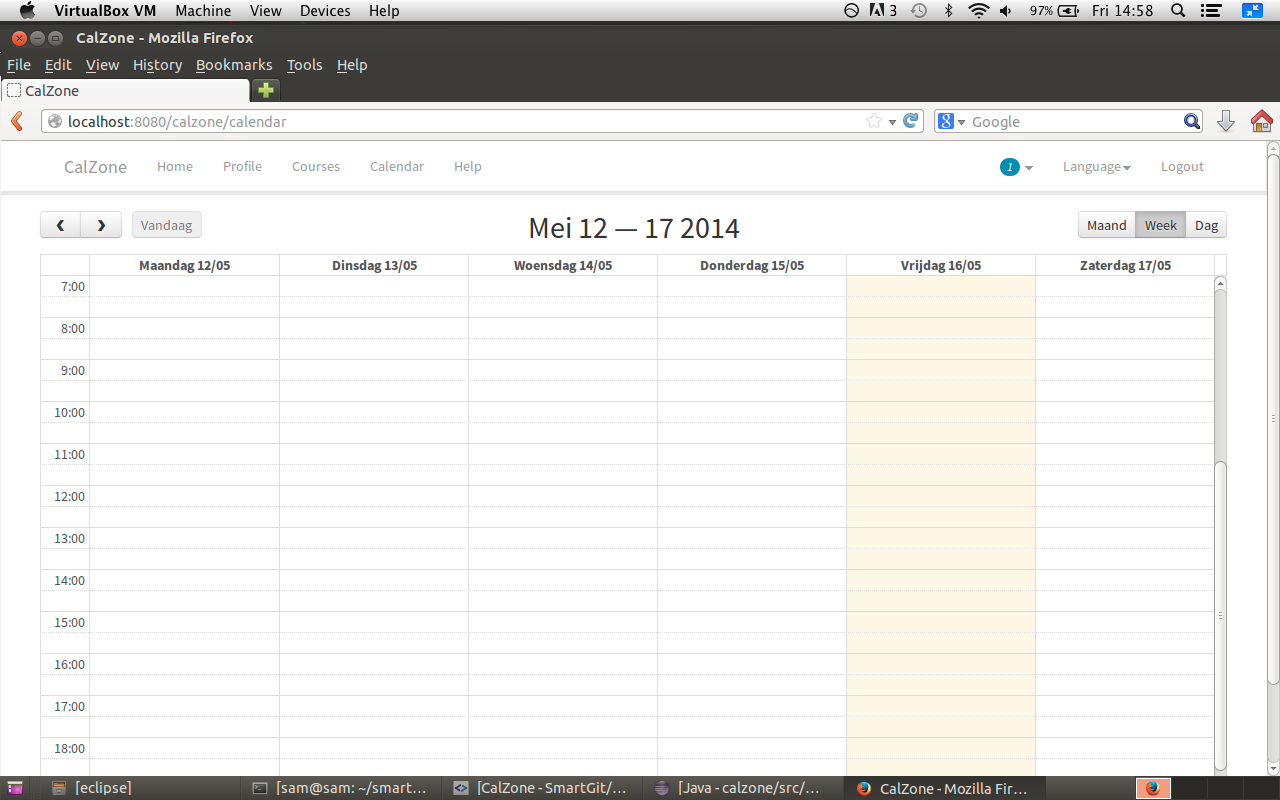
\includegraphics[scale=0.4]{img/CalzoneCalendar}}
\label{fig:CalZone Calendar}
\end{figure}
\end{center}


 
%Gespecializeerd schema opvragen lesgever.
\subsubsection{Gespecialiseerd schema opvragen lesgever}       
\noindent\begin{table}[H]
            \begin{tabular}{l | p{10cm}}
                \textbf{ID:} & FR5.5 \\ \hline
                \textbf{TITEL:} & Gespecialiseerd schema opvragen lesgever\\ \hline
                \textbf{PRIORITEIT:} &  Medium \\ \hline
                \textbf{PREREQUISITIES:} & \\ \hline
                \textbf{TOEGANG:} & Professor \\ \hline
                \textbf{BESCHRIJVING:} & Een professor kan zijn eigen schema van alle lessen bekijken die onder zijn bevoegdheid vallen. Ook WPO's die niet door de professor gegeven worden staan op deze speciale lijst. Verschil word aangeduid via kleurmarkeringen. \\ 
            \end{tabular}\\
            \caption{FR5.5 - Gespecialiseerd schema opvragen lesgever}
            \label{tab:FR5.5 - Gespecializeerd schema opvragen lesgever}
        \end{table}
        
\textbf{Stappenplan:}
\begin{enumerate}
\item De professor kan bovenaan in de navigatiebalk klikken op de knop "Geavanceerd schema".
\item Programma zoekt alle vakken, zowel hoor- als werkcollege die tot het vakkenpakket van de professor behoren en toont dit in een nieuw scherm.
\end{enumerate}